%========================================================================
\documentclass[11pt]{article}
\usepackage{graphics}
\graphicspath{{figs/}}

%===========================================
% Fix the margins
\setlength{\topmargin}{-0.4in}    % distance from top of page to begining of text
\setlength{\textheight}{9.0in}    % height of main text
\setlength{\textwidth}{6.5in}     % width of text
\setlength{\oddsidemargin}{0.in}  % odd page left margin
\setlength{\evensidemargin}{0.in} % even page left margin

%===========================================
\usepackage{amssymb,amsfonts}
\usepackage{amsmath}

%===========================================
\begin{document}

\title{Incompressible Navier Stokes equation using fractional step method}

\author{Zhengjiang Li}

\date{}

\maketitle

\section {Navier-Stokes equation system}

consider incompressible Navier-Stokes equation:

	$$ \frac{\partial u}{\partial t} + ( u \cdot \nabla) u = - \nabla p + \frac{1}{Re} \nabla^2 u $$

	$$ \nabla \cdot u = 0 $$

the discretization method here is finite volume algorithm on staggered mesh.

\begin{figure}[!h]
	\caption{p, u, v on staggered mesh}
	\centering
	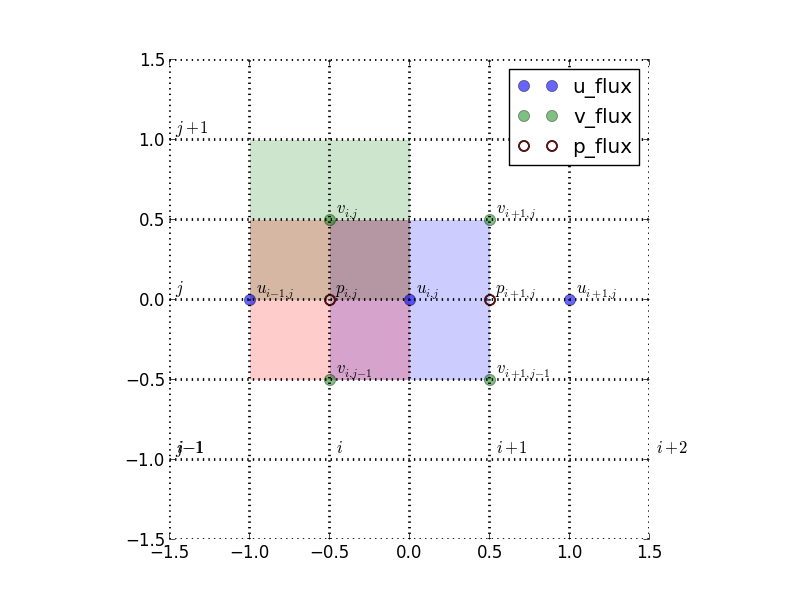
\includegraphics{staggeredmesh}
\end{figure}

where pressure DoF is interpolated at center of the cell, and velocity fluxes DoFs are interpolated at the wall of cell,respectively. The conservation equation in each cell satisfy:

$$ \frac{\partial}{\partial t} \int _{\Omega _{ij}} u dV = \int_{\partial \Omega_{ij}} ( -u^2 n_x - u v n_y - p n_x + \nu (u_x n_x + u_y n_y) ) dA  $$

The first term in a grid cell shown in figure above, can be evaluated as

$$  \frac{\partial}{\partial t} \int _{\Omega _{ij}} u dV = \frac{\partial}{\partial t} u_{i,j-1/2} h_x h_y $$

the convective term is defined on cell faces, while the averages must be used, which is then

$$  \int_{\partial \Omega_{ij}} u^2 n_x + u v n_y dA \approx = (\hat{u}_{i+1/2, j-1/2} ^ 2 - \hat{u}_{i-1/2, j-1/2}^2) h_y + ( \hat(v)_{ij} \tilde{u}_{ij} - \hat{v}_{i,j-1} \tilde{u}_{i,j-1}) h_x $$

and viscosity term is

$$ Vis_term = \frac{1}{Re}( \frac{1}{h_x^2} (u_{i+1,j} - 2u_{ij} + u{i-1,j}) + \frac{1}{h_y^2}( u_{i,j+1} - 2u_{i,j} + u_{i,j-1}) ) h_x h_y $$

As we see here, on staggered mesh for 2D problem, DoFs of pressure, u-fluxes, v-fluxes have different sizes as

\begin{center}
	\begin{tabular}{|l |l |l |l|}
	\hline
	Variable & Interiour resolution & B.C. included \\ \hline
	P	&  nx, ny & (nx+2), (ny+2) \\ \hline
	U	&  (nx-1), ny & (nx+1), (ny+2) \\ \hline
 	V	&  nx, (ny-1) & (nx+2), (ny+1) \\ 
	\hline
	\end{tabular}
\end{center}
  
where $nx,ny$ are the number of cells in x, y direction, respectively.

In details here, I use the implicit Crank-Nicolson(CN) integration for the viscous terms and the explicit second-order Adams-Bashforth(AB2) scheme for the convective terms, namely:

\begin{align*}
  \frac{v^{n+1} - v^n}{\Delta t} + [\frac{3}{2} H(v^n) - \frac{1}{2} H(v^{n-1}] \\
 = -G p^{n+1} + \frac{1}{2Re} L(v^{n+1} + v^n) + bc_1 
\end{align*}

$$ D v^{n+1} = 0 + bc_2 $$

The capital $H, G, L, D$ are AB2 operator, gradient operator, Laplace operator, and divergence operator, respectively. written in a system of equations:
$$ 
\begin{bmatrix} A && G \\ D && 0 \end{bmatrix} \begin{pmatrix} v^{n+1} \\ p^{n+1} \end{pmatrix} = \left( \begin{array}{c} r \\ 0 \end{array} \right) + \left ( \begin{array}{c} bc_1 \\ bc_2 \end{array} \right) $$
where

$$ A = \frac{1}{\Delta t} [ I - \frac{\Delta t}{2Re}L] $$

$$ r_{explicit term} = \frac{1}{\Delta t} [ I + \frac{\Delta t}{2Re} L] v^n - [\frac{3}{2} H(v^n) - \frac{1}{2} H(v^{n-1}] $$

consider fluxs and discrete pressure as the primary variables, introduce $ R^{-1}q = v $ in the equation above.

$R$ is the dialogal matrix of x-spacing, y-spacing in each cell.

Note that the boundary conditions have already been incorporated at this point, teh exact forms of matrics $L, D, G$ are depent on the boundary conditions, the unknowns $qx, qy, p$ refer to only those nodes in the interior of the domain.

\section{fractional step method}

For an algebraic system of equation above,to remove the singularity,  Blair Perot had given the Block LU Decompositon method, as we can approximate the momentum equation by approximation the pressure term, as 

 $$ 
\begin{bmatrix} A &&  (AB^N)G \\ -G^T &&  0 \end{bmatrix} \begin{pmatrix} q^{n+1} \\ \phi ^{n+1} \end{pmatrix} = \left( \begin{array}{c} r_{explicit term} \\ 0 \end{array} \right) + \left ( \begin{array}{c} bc_1 \\ bc_2 \end{array} \right) $$

where $ -G^T = D$

then, decomposition as:

$$ 
\begin{bmatrix} A && 0 \\ -G^T && G^TB^NG \end{bmatrix} \begin{pmatrix} q^* \\ \phi ^{n+1} \end{pmatrix} = \left( \begin{array}{c} r \\ 0 \end{array} \right) + \left ( \begin{array}{c} bc_1 \\ bc_2 \end{array} \right) $$

$$ 
\begin{bmatrix} I &&  B^NG \\ 0 && I \end{bmatrix} \begin{pmatrix} q^{n+1} \\ \phi ^{n+1} \end{pmatrix} = \left( \begin{array}{c} v^* \\ p^{n+1} \end{array} \right) $$

in equations, it looks like the following:

\begin{align}
	A q^* = r + bc_1;
	\\ G^TB^NG \phi ^{n+1} = G^Tq^* + bc_2 ;
  	\\ q^{n+1} = q* - B^NG \phi ^{n+1};
\end{align}

where matrix $B$ is an approximation of $A^{-1}$, using the Taylor series expansion of $A^{-1}$, we have:
	$$ A^{-1} \approx B^N = \Delta t M^{-1} $$

In this projection system, define two right hand side(rhs) vectors in consistant with intermediate velocity equation and Poisson equation,respectively. 
\begin{align}
	rhs1 = r_{explicit term} + bc1
\\	rhs2 = G^T q^* + bc2
 \end{align}

$bc1$ is the boundary values for momentum equation. e.g. consider left (-X inlet) boundary, and center difference for laplacian operator.

$$ \frac{u_{i,0}^{n+1}}{\Delta t} - C_{implicit} (4u_{i,0} - u_{i+1,0} - u_{i-1,0} - u_{i,1} - u_{i,-1}) = r_{explicit term} $$

$u_{i,-1}$ is derived from the boundary value from inlet velocity boundary, which is the known value, so put it on the right hand side, and called it $bc_1$.

similar for $bc2$ in divergence equation, which is the known fluxes at boundary.

One more thing, as all pressure nodes are interior to the domain, there is no boundary conditions on pressure. All given boundary values are acted only on $x,y$ fluxes in the walls, and for simple implementation, here only Dirichlet velocity boundary is considered, except at the outlet of the domain, we take Newman boundary(satisfy convective condition),as with given both inlet/outlet velocity profile is too strict condition. 

\section{Building Matrix and Vectors}

The matrix used in this system, are $A, B^NG, G^T, R$.

\begin{enumerate}

\item{ matrix $A$ }

Each part of Matrix $A$ is basically a Laplacian Matrix multifly a scalar, and then minus the unit matrix. For interior points, it's easy to insert the 5 values simutaniously, while for near boundary points, as $bc1$ is already moved to righ hand side, the full 5-points is reduced to 4-points or 3-points stencils, when the current point is exactly on the corner of the domain.

for example, $u-fluxes$ brings $A_{11}$ with size $ (nx-1) \cdot ny $ in each direction, and $v-fluxes$ brings $A_{22}$ with size $nx \cdot (ny-1)$ in each direction. And as the viscostiy term, in which there is u-v product,is moved to rhs, so the cross-term matrix $A_{12}, A_{21}$ are null space, which can be done automatically by MatNullSpaceCreate. 

Define $n1= (nx-1) \cdot ny $, $n2 = nx \cdot (ny-1) $, $q=[]_{(n1+n2),1}$

$$ 
\begin{bmatrix} A^{11}_{n1 \cdot n1} &&  A^{12}_{n2 \cdot n1}  \\ A^{21}_{n1 \cdot n2} && A^{22}_{n2 \cdot n2}  \end{bmatrix} \begin{pmatrix} u^{n+1} \\ v^{n+1} \end{pmatrix} = \left( \begin{array}{c} rhs_1 \\ rhs_2 \end{array} \right)$$


\item{matrix $G$ }

This Matrix is mapping to pressure with size $nx \cdot ny$ in cols direction and the rows size is same as Matrix $A$. 
 
Define $n3 = nx \cdot ny $, so $ P = []_{n3,1}$

$$ B^N = [  ]_{ (n1+n2) \cdot (n1+n2)} $$
$$ G = [ ]_{(n1+n2) \cdot n3} $$

\item{Vec $rhs$}

From the matrix equations above, we can easily see the size of $rhs_1 = n1 + n2$, and the size of $rhs_2 = n3$, both make sense as we said before, the $bc1$ is boundary for momentum equations, adn $bc2$ is boundary for divergence equation, where pressure is not explicit,but play the role as a Lagrangian multiplier. 

\end{enumerate}


\section{Implement in Petsc}

For a 2D recantgular domain, first define $DMDA$ for both pressure and x-flux, y-flux, as $pda, uda, vda$, create all corresponding global vectors, and the matrix as in last section.For initial values and boundary values, call $initialFluxes$ and $updateBoundaryGhosts$, respectively.

As known matrix $A, B^NG, R$ are all pre-defined, they need to assemble once and for all, while in $rhs1 = r^n + bc_1$, no doubt explicit term $r^n$ should be updated in each timestep, and $bc_1$ is need to be update for top/bottom wall for $u_{fluxes}$ and right/left wall for $v_{fluxes}$, respectively, since in these places we don't have an exact boundary values for the time on the staggered mesh. Same for $rhs_2 = G^T q^* + bc_2$, as $q^*$ is updated everytime step, as well as $bc_2$ on staggered mesh.

so in every timestep, we do two-steps. In step one, we update $rhs_1$ and call $ksp1$ to solve the $IntermediateVelocity$; in step two, we update $rhs_2$ and call $ksp2$ to solve the $PressurePoisson$, and additional step is $projection$ to update the velocity.

And that's it. and the easility of using projection method is appareant, that it only need ksp linear solver and for more complex cases, when dealing with immersed boundary force, this method still works great.

\section{Results \& Analysis}


\section{petsc src}

\section {Reference}
1 An analysis of the fractional step method, J. B. Perot 1993
\\ 2 Analysis of an exact fractional step method, W. Chang 2002
\\ 3 Lectures in computational fluid dynamics of incompressible flow: mathematics, algorithms and implementations, J. M. McDonough 2007

\end{document}
